\documentclass[a4paper,10pt,bibtotoc]{scrartcl}
\usepackage{a4wide,usg}
\usepackage{draftcopy}

%% Do NOT remove: required to extract SVN information
\svnInfo $Id$

%% Adjust page footer
\fancyfoot[LE,LO]{LOFAR-USG-ICD-008: Rotation Measure Synthesis Cubes}
\fancyfoot[RE,RO]{\textsc{lofar} Project}

\begin{document}

%%_______________________________________________________________________________
%% Titlepage

\title{LOFAR Data Format ICD \\ Rotation Measure Synthesis Cubes \\
{\normalsize Document ID: LOFAR-USG-ICD-008} \\ 
{\normalsize Version 0.07.11} \\
{\normalsize SVN Repository Revision: \svnInfoMaxRevision}}
\author{J.~Anderson, L.~B\"ahren, M.~Bell, T.~Riller, K.~Anderson}
\date{\small{SVN Date: \svnInfoDate}}
\maketitle

\tableofcontents
\listoffigures
\listoftables
\clearpage

%%_______________________________________________________________________________
%% Change record of the document

\section*{Change record}
\addcontentsline{toc}{section}{Change record}

\begin{tabular}{lllp{10cm}}
  \hline
  \sc Version & \sc Date & \sc Sections & \sc Reason \\
  \hline \hline
  0.01.00  & 2010-06-02 & All & Initial version \\
  0.02.00  & 2010-06-04 & Appendix & Removed section ``Coordinate group examples''
  from the appendix; detailed description and examples now can be found in
  \texttt{LOFAR-USG-ICD-002} (``Representation of World Coordinates'') \\
  0.03.00 & 2010-07-15 & All & Incorporated James Anderson's comments from the
  forum. \\
  0.04.00 & 2010-12-07 & All & Using \LaTeX\ package \texttt{hyperref} for
  references, enabling better navigation through the document and access to
  external resources. Put back in usage of \texttt{a4wide} package, in order to
  make the textbox consistent with that of the other ICDs. \\
  0.05.00 & 2011-01-04 & All \ref{sec:organization of the data}, \ref{sec:detailed structure} &
  Review, cleanup, and overhaul, new diagram illustrating the latest design. \\
  0.05.01 & 2011-01-17 & --- & Minor revision, activation of svn keywords. \\
  0.05.02 & 2011-01-18 & \ref{sec:organization of the data}, \ref{sec:rmsf group} & Correction
  of fontsize. Adjusted attribute names. \\
  0.06.00 & 2011-01-19 & All & Removed several poorly defined and at the moment extraneous groups. Now focusing on the basic requirements for the description of a RMSC. Added a polarization coordinate group. \\
  0.07.00 & 2011-02-01 & \S \ref{sec:overview} & move and insert image table, descr. text\\
  0.07.01 & 2011-03-10 & all & Maintain list of references through Bib\LaTeX\ database. \\ 
  0.07.02 & 2011-03-15 & all & Fixed some typos and changed all group and attribute names so that they are UPPER\_CASE rather than CamelCase. \\
  0.07.03 & 2011-07-06 & all & Matching up group type attributes and
  notation; consolidation of labels to refer to standard sections
  and tables. \\
  0.07.04 & 2011-09-20 & \ref{sec:organization of the data} & Update of
  Fig.~\ref{fig:high-level structure} \\
  0.07.05 & 2011-09-28 & all & Change data types of attributes: \verb|float|
  $\rightarrow$ \verb|double|. \\
  0.07.06 & 2011-10-25 & all &  Use names 
\verb|PROCESS_HISTORY| and \verb|SYS_LOG| consistently throughout the document. 
  Change data type of attributes: \verb|bool| $\rightarrow$ \verb|unsigned int|. \\
  0.07.07 & 2012-01-10 & all &   
  Change data type of attributes: \verb|unsigned int| $\rightarrow$ \verb|bool|;
  added input tex file on types to the section just before Acknowledgements.
  Changed the svnInfoRevision to svnInfoMaxRevision, in order to take the sub-tex file changes into account for the latex compile.\\
  0.07.08 & 2012-02-06 & \ref{sec:detailed structure} & Added matadata\_intro.tex file 
  to explain optional header keys.  No keywords were made optional within the tables, 
  since it is not yet clear which keys are not required.\\
  0.07.09 & 2012-02-21 & all & Fixed all quotes for correct forward/backwards orientation. \\
  0.07.10 & 2012-03-06 & cover & Added draftcopy package for background 'draft' text.\\
  0.07.11 & 2012-04-03 & all & Removed Sec. 5 (Interfaces) and added a list of figures and tables. \\

  \hline
\end{tabular}

\input version_numbering

\input types

\input notation

\subsection*{Acknowledgements}

The document was originally developed by K.~Anderson in collaboration
with L.~B\"ahren.

\clearpage

%% _______________________________________________________________________________
%% Introduction

\section{Introduction}
\label{sec:introduction}

\subsection{Purpose and Scope}
\label{sec:purpose and scope}

This document sets forth a formal data interface specification for LOFAR data products.  The specification applies to data structures produced by various LOFAR processing pipelines that will be called \textsl{Rotation Measure Synthesis Cubes} (henceforth RMSC).  This is a specification for RMSC data products only and in no way implies, and should not be inferred as, a specification for any data structures the project may use during \textit{in situ} processing by way of producing a final standard Rotation Measure Synthesis Cube file.

This document is intended to be the formal interface control agreement between the LOFAR project, observers/users of LOFAR data products, and the eventual LOFAR science archive facility.

\subsection{Context and Motivation}
\label{sec:context and motivation}

A RMSC file will be the data hosting structure for LOFAR RM synthesis output data. It is therefore incumbent on the LOFAR project to define and describe the structure of the LOFAR RMSC file format, and how the various data types are defined and described within the context of that format.

While image hypercubes are the primary data product of the RM synthesis pipeline, they are accompanied by a number of by-products, such as flagging information, CLEAN components, local and global sky models (LSM, GSM), etc.  In the  more traditional approach, where all such products are stored and managed separately, a large amount of book-keeping is required to maintain consistency.  For the LOFAR project, a RMSC file product will be defined within the context of  the Hierarchical Data Format 5, or HDF5. HDF5 allows for storage, not only of the data, but for the associated and related meta-data describing the RMSC contents, conditions of observations, etc. As an "all-in-one" wrapper, the HDF5 format simplifies the management of what are expected to be very large datasets that formats such as FITS cannot pragmatically accommodate.

% There has been much discussion of a putative need for LOFAR file headers to adhere to FITS-like header keywords.  Though it is envisioned that the LOFAR project will provide observers and other users with FITS format image files upon request, it is not entirely necessary that HDF5 header keywords match FITS keyword conventions in a LOFAR RMSC file itself.  A format conversion layer can certainly be developed to provide rigorous transformation of LOFAR headers into more restricted FITS header keyword sets. However, development of such a layer would be simplified in the event that LOFAR RMSC files make use of de facto FITS standard keywords as much as possible.

For the purposes of further discussion regarding RMSC file adherence to FITS keyword standards, the \textit{ESO Data Interface Control Document}, has been adopted as the FITS keyword model.

\input applicable_documents

%% ______________________________________________________________________________
%%                                                              Section: Overview

\section{Overview}
\label{sec:overview}

LOFAR imaging data will be presented in a number of LOFAR data formats, all of which will provide data arrays of differing dimensions, depending upon the respective observation.  Sky Image Cubes, Rotation Measure Cubes, Near-field cosmic ray images (``CR image'' in Table \ref{tab:lofar_data_types}), etc., all have different dimensions and coordinate types.  Table \ref{tab:lofar_data_types} illustrates the various image data array dimensions  that LOFAR imaging may produce.

\input coordinates_image_table

Each data type is described in detail by an appropriate interface control document.  This document pertains to, and describes only those data conforming to the LOFAR datatype "RMSC" (Rotation Measure Synthesis Cube).  The dataset array in a RMImage Cube will be a \verb|ndarray| data structure, as can be created by the C-based  \textit{numarray/numpy} Python packages. The Rotation Measure Synthesis Cube is designed to store the 3D polarized intensity data produced from the LOFAR RM synthesis pipeline.  The nominal dimensionality of a RMSC \texttt{DATA} group's dataset will be 4 (\texttt{NAXIS=4}), wherein the image cube (or cubes) will be defined in (C-type order) \textit{Polarization}, \textit{Faraday Depth}, \textit{Dec}, \textit{RA}, as shown in Table \ref{tab:lofar_data_types}

This document is structured as follows: Section \ref{sec:organization of the data} will present a high-level view of the hierarchical structure of LOFAR data files, file form, and semantic conventions the interface will adhere to, including a statement of the primary data product format, HDF5. These conventions will also include names, meaning, and physical units that may be used to generate and interpret the data files.  Section \ref{sec:detailed structure} will present the low-level specification for the data, including a description of the structure of LOFAR RM Synthesis Cube files, and the various group entities and sub-structures comprising these RMSC data files, i.e. LOFAR group types, units, physical quantities. Finally, the LOFAR filename convention appears in Appendix~\ref{sec:filenames}, and Coordinate group examples are present in Appendix~\ref{sec:coordinate examples}.

%% _______________________________________________________________________________
%% Organization of the data

\section{Organization of the data}
\label{sec:organization of the data}

\subsection{High level LOFAR RM Synthesis Cube file structure}

A LOFAR Rotation Measure Synthesis Cube (RMSC) file will adhere to the following guidelines:

A LOFAR RMSC file (a hypercube image file) is herein defined within the context of the Hierarchical Data Format, version 5 (HDF5) .  In an effort to minimize the hierarchical depth of the file structure, a RMSC file is designed to be as "flat" as possible, providing access to the necessary data without undue hierarchical tree crawling.

Therefore, the RMSC file structure will comprise a primary group, a "root group" in HDF5 nomenclature, which may be considered equivalent to a primary header/data unit (HDU) of a standard multi-extension FITS file.  This primary group will consist only of header  keywords (``attributes'' in HDF5 nomenclature) describing general properties of an observation, along with pointers to contained subgroups.  These subgroups will comprise a ``System Log,'' as well as a single ``RMIMAGE'' group (\textit{see \S\ \ref{sec:rm_image group}}), where an \texttt{RMIMAGE} group will contain data and meta-data for a specified set of Faraday depths. 

\begin{figure}[htbp]
  \centering
  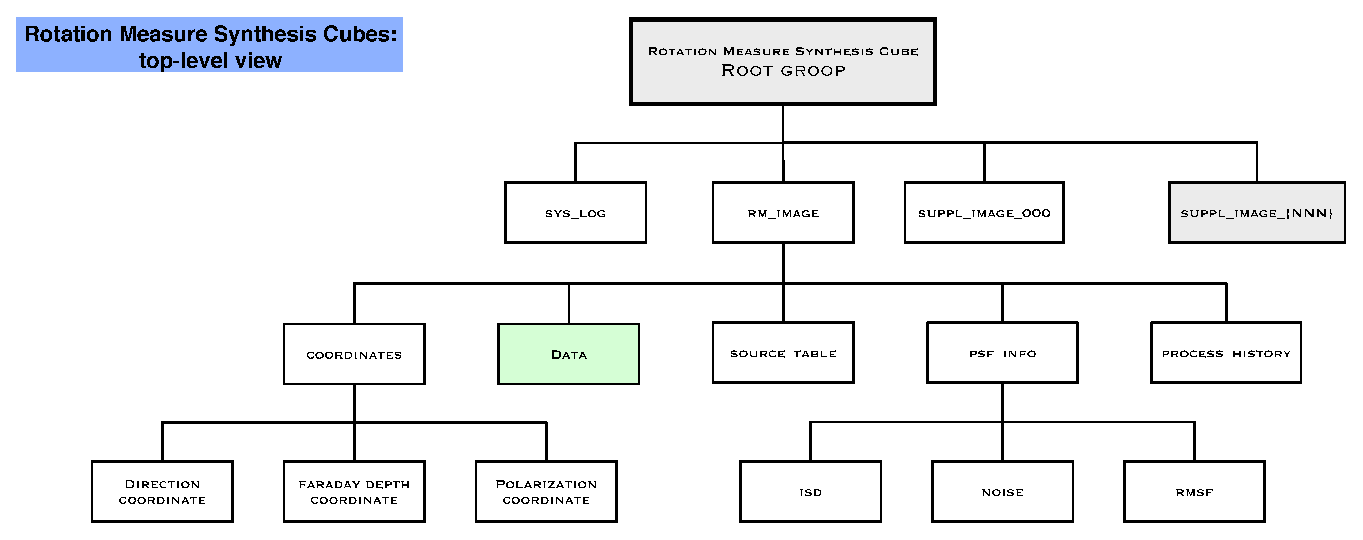
\includegraphics[width=\textwidth]{figures/RMSC_TopLevelView.eps}
  \caption{Rotation Measure Synthesis Cube (RMSC) file structure}
  \label{fig:high-level structure}
\end{figure}

Unlike the SkyImage Cube, a LOFAR RMSC file will \textit{only require a single RMImage group}. Separation in to ``sub-bands'', each having different properties, is unnecessary.

The structure of an RMSC file can be represented through HDF5 as a \textsc{posix}-style hierarchy\footnote{$\mathtt{<...>}$ Indicates optional or potiential subgroups, where only one coordinate subgroup of any type shall be present in a LOFAR RMSC file.}

\begin{lstlisting}
OBSERVATION/
OBSERVATION/SYS_LOG
OBSERVATION/RMIMAGE/
OBSERVATION/RMIMAGE/COORDINATES
OBSERVATION/RMIMAGE/COORDINATES/<DIRECTION_COORD>
OBSERVATION/RMIMAGE/COORDINATES/<FARADAY_DEPTH_COORD>
OBSERVATION/RMIMAGE/COORDINATES/<POLARIZATION_COORD>
OBSERVATION/RMIMAGE/DATA
OBSERVATION/RMIMAGE/SOURCE_TABLE
OBSERVATION/RMIMAGE/PROCESS_HISTORY
OBSERVATION/RMIMAGE/PSF_INFO
...
\end{lstlisting}

\subsection{Overview of RMSC Groups}

A LOFAR RMSC file will then comprise \verb|SYS_LOG| group just below the root level which contains logs and parameter files which are relevant to the entire file.  Additionally, just below the root level, the RMSC file will contain a \textit{single} \texttt{RMIMAGE} group containing a \texttt{DATA} group, a \texttt{COORDINATES} group, a \verb|SOURCE_TABLE| table, a \verb|PSF_INFO| group and a \verb|PROCESS_HISTORY| group, which contains pertinent logs and parameter sets of the relevant image.

These main building blocks of the RMSC HDF5 file are:

\begin{enumerate} \parskip 0pt
\item \textbf{File Root Group} (\verb|ROOT|). The root level of the file contains
  the majority of associated meta-data, describing the circumstances
  of the observation. These data attributes include time, frequency
  and other important characteristics of the dataset. See
  Sec.~\ref{sec:root group} for a detailed description.
  
\item \textbf{System Logs Group} (\verb|SYS_LOG|). This is a catch-all
  envelop encapsulating information about all the system-wide steps of
  processing which are relevant to the entire observation, such as
  parameter sets and processing logs. See Sec.~\ref{sec:sylog group}
  for a detailed description.
  
\item \textbf{RMImage Group}. The \texttt{RMIMAGE} group contains its own set of five (5) sub-groups.  Characteristics about the Rotation Measure Image are stored as Attributes in group headers.  The \texttt{RMIMAGE} group will contain one (1) \texttt{DATA} group, which will in turn contain one (1) dataset as an ndarray, along with associated attributes.

%\item \textbf{Supplemental Image Group (SIG)}.  A Suppplemental Image Group will hold various supplementary image products necessary to the further analysis of the rotation measure synthesis data.  These SIGs are expected to contain images that otherwise cannot be derived from contained data, will use Stokes I direction axes, NOT faraday depth axes.\footnote{Based Rotation Measure Synthesis Cubes (RMSC) ICD Discussion NOTES, 10.11.2010, J. Anderson, K. Anderson, L. Baehren, M. Bell, T. Riller}

\item \textbf{Source Tables}.  A \verb|SOURCE_TABLE| Table  will contain a table of the sources listed in a processing file, a \verb|.skymodel| file.  Attributes will describe the columnar data.  This table will also contain the model components obtained from one of several possible types of imaging routines (e.g. CLEAN, Wavelet, etc.).

\item \textbf{Coordinates Groups} (\verb|COORDINATES|). The \texttt{RMIMAGE} group contains one \texttt{COORDINATES} group, which stores the relevant world coordinate conversions. The Coordinates group \textit{must contain at least one subgroup} of the kind direction and Faraday depth.  Multiple coordinate subgroups are permissible as needed, but only one of any type can be present in a LOFAR RMSC file. The \texttt{COORDINATE} group will contain 3 or $3 \times N$ Coordinate sub-groups. 
  
\item \textbf{Processing History Groups} (\verb|PROCESS_HISTORY|)
  can be found on the \texttt{RMIMAGE} level. These are catch-all
  envelops encapsulating information about all the steps of
  processing, such as parameter sets and processing logs. See
  Sec.~\ref{sec:processing history group} for a detailed description.

\item \textbf{Data Group/Data arrays} (\verb|DATA|). The rotation measure synthesis image data are stored as ndarrays in the respective \texttt{DATA} group - it is at this 3rd hierarchical depth where the image data reside. The data storage options are still being investigated, in order to determine the maximum efficiency of data seeks and file I/O. 

\item \textbf{PSF Info Groups}. The \verb|PSF_INFO| group is a subgroup of the \texttt{RMIMAGE} group and contains information about the \textbf{point spread function} (PSF) in both the sky plane and along the Faraday depth axis. This includes the basic dimensions of the PSF, the full 1-D PSF in Farday depth, and the list of frequencies and channel widths from which the Faraday depth PSF has been derived.

\end{enumerate}

%% _______________________________________________________________________________
%% Detailed Data Specification

\section{Detailed Data Specification}
\label{sec:detailed structure}

\input metadata_intro

\subsection{The Root Group ({\tt ROOT})}
\label{sec:root group}

The LOFAR file hierarchy begins with the top level \verb|`ROOT'| group.  This is the file entry point for the data, and the file node by which navigatation of the data is provided.  The \texttt{ROOT} group will comprise a set of attributes that describe the underlying file structure, observational metadata, the LOFAR image data, as well as providing hooks to all groups attached to the \texttt{ROOT} Group.   

This section will specify two sets of attributes that will appear in the \texttt{ROOT} group: a set of \cla\ (CLA) that will be common to all LOFAR science data products, and a set of attributes that are specific to LOFAR RMSC data.  Though these attributes will all appear together in the \texttt{ROOT} attribute set, they are separated in this document in order to demarcate those general LOFAR attributes that are applicable across all data, and those attributes that are \texttt{RMIMAGE}-specific.
In other words,

\begin{verse}
  \verb|Root Attributes = Common LOFAR Attributes (CLA) + Supplemental RMSC Root Attributes.|
\end{verse}

The {\cla} are the first attributes of any LOFAR file root group.

%%_______________________________________________________________________________
%%                                                        Common LOFAR Attributes

\subsubsection{\cla}
\label{sec:common lofar attributes}

This section will specify a set of attributes that will be common to
LOFAR science data products.  These ``\cla'' will
appear as attributes at the root level of all LOFAR data files.
\textit{All} LOFAR data products, including RMSC \textit{inter
  alia,} will share a common set of metadata root-level attributes.
These \cla\ are to be the first set of attributes of
any LOFAR file root group.

Table~\ref{tab:lofar common metadata} lists the {\cla} (CLA) which can be found in all LOFAR data file types.  These Attributes are required to be in the Root Group; if a value is not available for an Attribute, a \verb|`NULL'| maybe used in its place.\\

\input lofar_common_metadata

\begin{table}[ht]
  \centering
  \begin{tabular}{|lrp{6cm}|} 
    \hline
    \sc \textbf{General LOFAR Group} & \sc \textbf{Value} & \textbf{Description} \\
    \hline
    Root          & \verb|`Root'|    & Top-level LOFAR group type \\
    System Log    & \verb|`SysLog'|  & System log files, parsets \\
    SIG*  				& \verb|`SIG'| & Supplemental Image Group \\
    \textbf{RMImage} & \verb|`RMImage'|   & RMImage group \\
    \hline \hline
    \sc \textbf{RMImage Group Subgroups} & \textbf{Value} & \textbf{Description} \\
    \hline
    Data group  & \verb|`rmscData'| & RMSC Data group (dataset) \\
    Source table & \verb|`SourceTable'| & Source List table  \\
    % Image Model table & \verb|`ImModTable'| & Image Model table  \\
    Processing History group &\verb|`ProcessHist'| & Processing History group \\
    Masks group* & \verb|`Masks'| &  Masks group \\
    PSF Info Group &\verb|`PSFInfo'| & PSF information group \\
    \textbf{Coordinates Group} & \verb|`Coordinates'| & Coordinates group \\
    \hline
    \sc \textbf{Coordinates Group Subgroups} & \textbf{Value} & \textbf{Description} \\
    \hline
    Direction coord group &\verb|`DirectionCoord'|& Direction coordinate group \\
    % Linear coord group      &\verb|`CoordLinear'|      & This is a linear coord group \\
    Faraday depth coord group   &\verb|`FaradayDepthCoord'|  & Faraday depth coordinate group \\
    Polarization coord group    &\verb|`PolarizationCoord'|    & This is a Polarization coord group \\
    \hline
    *\textit{Proposed groups under advisement.} & & \\ 
    \hline
  \end{tabular}
  \caption{LOFAR RMSC Group Types}
  \label{tab:group types}
\end{table}

\subsubsection{Supplemental RMSC Root Attributes} The root group of a LOFAR RMSC file will comprise header attributes, various subgroups as indicated above, and appropriate pointers to the root-level of a single \verb|RMIMAGE| sub-group, which contains the relevant data and meta-data for a specified set of Faraday depths.

This root group header will comprise general information about the observation itself, sparing relevant data details for the headers of the lower order sub-groups.  Table \ref{tab:attributes root group} presents additional root group attributes for a LOFAR RMSC file that do not appear in the LOFAR common metadata table.\footnote{\textbf{ *} Indicates attributes that may \textit{migrate from the root group} and be broadcast to the \texttt{RMIMAGE} group.  Recent observations have indicated that different sub-bands potentially can have different integration times.}

\begin{table}[htbp]
    \centering
    \begin{tabular}{|llrl|}
        \hline 
        \sc Field/Keyword     & \sc Type      & \sc Value & \sc Description \\
        \hline \hline 
        \small{\verb|IMGROUPS|}      & \verb|bool| & \verb|`true'| & File has RMImage subgroups \\
        \small{\verb|NOF_IMAGES|}  & \verb|int|   & \verb|`1'| & \small{\texttt{1}} RMImage group in this file \\
        \small{\verb|TARGET_RA |}  & \verb|double| &                & \small{\texttt{RA}} of \small{\texttt{TARGET}} (at LOFAR core)\\
        \small{\verb|TARGET_DEC|}  & \verb|double| &                & \small{\texttt{Dec}} of \small{\texttt{TARGET}} (at LOFAR core)\\
        \small{\verb|INPUT_FILE|}  & \verb|string|  &                & Input data file (SkyImage Cube) \\   
        \hline
    \end{tabular}
    \caption{Additional Root group attributes, LOFAR RMSC}
    \label{tab:attributes root group}
\end{table}

%%_______________________________________________________________________________
%% Subsection: The System Logs Group (SYS_LOG)

\input groups_sys_log

%%_______________________________________________________________________________
%% Subsection: The RMImage Group

\subsection{The RMImage Group}
\label{sec:rm_image group}

The \texttt{RMIMAGE} group will be an HDF5 group serving as a container for the five sub groups described below. A \texttt{RMIMAGE} group is designed to be as complete and self-contained a Rotation Measure Synthesis cube as possible.  It will contain relevant data and metadata for a processed cube of polarized intensity as a function of Faraday depth (known as the Faraday dispersion function).  However, any breakout protocol will be required to inherit some or all root group attributes in order to function as a stand-alone image.  The adopted form allows for relatively simple extraction and conversion in a FITS-compatable form. 

\begin{figure}[htbp] 
 \begin{center}
    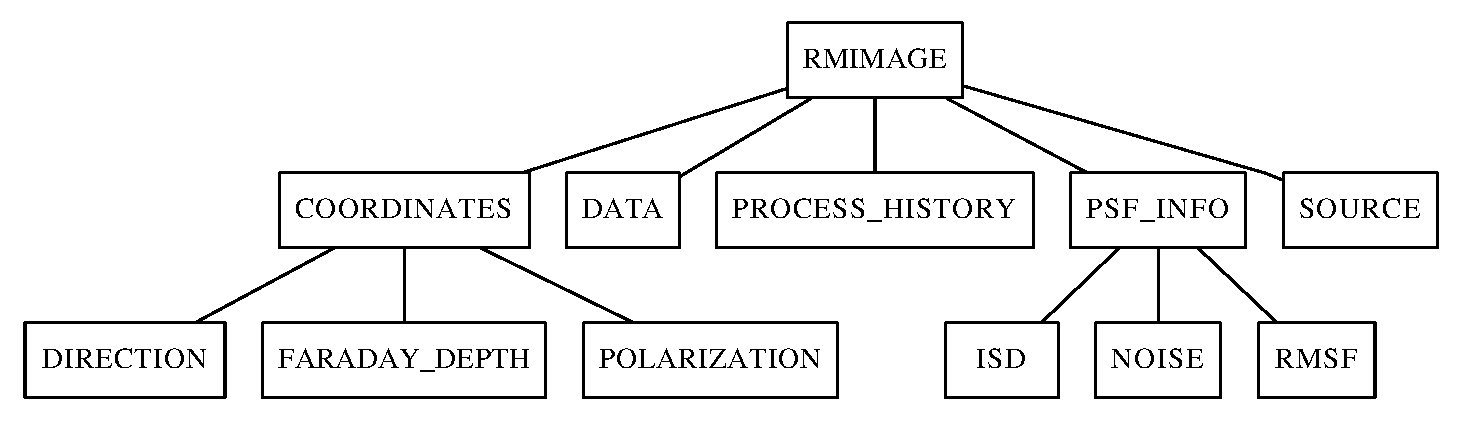
\includegraphics[scale=0.48]{./figures/rm_image.eps}
  \end{center}
\caption{\texttt{RMIMAGE} Group structure}
\end{figure}

A \texttt{RMIMAGE} group will comprise five sub groups.  These five groups, two hierarchical levels below the root group� in a LOFAR RMSC \textit{(Fig. 1)}, will be

\begin{itemize}
\item A \texttt{COORDINATES} group that will contain \texttt{FARADAY\_DEPTH\_COORD}, \texttt{DIRECTION\_COORD} and \texttt{POLARIZATION\_COORD} subgroups that describe the axes of the associated dataset.
\item A \texttt{DATA} group that will contain a dataset array.
\item A \verb|SOURCE_TABLE| table that will be a tabular representation of a Local Sky Model as well as any image model component (e.g. CLEAN) information.
\item A \verb|PROCESS_HISTORY| group, which will be a meta-data container holding various processing products such as log files, parameter sets, RFI mitigation tables, etc..
\item A \verb|PSF_INFO| group, which contains information about the point spread function in both the image plane (i.e. the CLEAN beam) and along the Faraday depth axis (i.e. the RM Spread Function). The full RM spread function may be stored here (in 1-D for the time being).
\end{itemize}

The table of \texttt{RMIMAGE} group attributes, table \ref{tab:RMImage group Attributes}, is notably sparse here and the reader must bear in mind that the Coordinates groups will contain most of the rest of the relevant Image group metadata (\textit{see \ref{sec:coordinates group}, ``Coordinates group''})

\begin{table}[ht]
  \centering
  \begin{tabular}{|lllrl|}
    \hline
    \sc Field/Keyword & \sc H5Type & \sc Type & Value &\sc Description \\
    \hline \hline
    \small\verb|GROUPTYPE|    & Attr. 
                              & \small\verb|string|
                              & \verb|`RMIMAGE'|
                              & \small{\texttt{LOFAR}} group type \\
    \small\verb|RMIMAGE|      & Attr.
                              & \small\verb|string|
                              & \verb|`RMImage_{NNN}'|
                              & Name of the image group. \\ 
    \small\verb|COORDINATES|  & Attr.
                              & \small\verb|string|
                              & ---
                              & name of \verb|`Coordinates'| subgroup  \\
    \small\verb|DATA|         & Attr.
                              & \small\verb|string|
                              & ---
                              & name of \verb|`Data'| subgroup \\
    \small\verb|SOURCE_TABLE| & Attr.
                              & \small\verb|string|
                              & ---
                              & name of \verb|`Source'| subgroup \\
    \small\verb|PROCESS_HIST| & Attr.
                              & \small\verb|string|
                              & ---
                              & name of \verb|`ProcessHist'| subgroup \\  
    \small\verb|PSF_INFO|     & Attr.
                              & \small\verb|string|
                              & ---
                              & name of \verb|`PSFInfo'| subgroup \\
    \hline \hline
    \small\verb|COORDINATES|     & Group \\
    \small\verb|DATA|            & Dataset \\
    \small\verb|SOURCE_TABLE|    & Dataset \\
    \small\verb|PSF_INFO|        & Group \\
    \small\verb|PROCESS_HISTORY| & Group \\
    \hline
  \end{tabular}
  \label{tab:RMImage group Attributes}
  \caption{Components of the RMImage group.}
\end{table}


\subsection{The Coordinates Group (\tt COORDINATES)}
\label{sec:coordinates group}

Coordinate information within a LOFAR RMSC file will exist in what is called a \texttt{COORDINATES} group, which will act as a container for a number of \texttt{COORDINATES} group objects.  The \texttt{COORDINATES} group will be a subgroup of an \texttt{RMIMAGE} group container, and may contain one or more subgroups that will describe relevent axes of the coordinates' associated \texttt{DATA} group using one or a combination of coordinate subgroups, where the enumerated are \texttt{direction, faraday depth, polarization}.

\input coordinates_group_table

The attributes presented in Table \ref{tab:coordinates-group} summarize the overall characteristics of the set of coordinates collected within this group:
\begin{itemize}
    \item \verb|GROUPTYPE| -- Identifier for the type of group, \verb|`Coordinates'|.
    \item \verb|NOF_COORDINATES| -- The number of coordinate objects/groups contained within the coordinates group.  For RMSC files, \verb|NOF_COORDINATES| will be 2, with one coordinate of type \verb|`DirectionCoord'|, and one coordinate of type \verb|`FaradayDepthCoord'|.
    \item \verb|NOF_AXES| -- The number of coordinate axes associated with the coordinate objects. Keep in mind, that a coordinate can have multiple (coupled) axes:  e.g. a direction coordinate is composed of two axes.
\end{itemize}

The layout of the embedded sub-groups will depend on the type of coordinate, of which there are several types.

\begin{comment}
  The description of the coordinates groups needs some major cleaning
  up: a) How many axes and coordinates are there for a RM Synthesis
  Cube? b) What is the ordering of the coordinate axes? c) Some of the
  description below appears to come from the Sky Cube ICD and might
  not be required here.

  Mike: There are three coordinate axes - Dec., RA, FD.  This should
  be the order. An optional spectral coordinate would contain
  information about the input spectral distribution (although this
  ideally belongs in the PSF information group if possible since it
  determines the RMSF and is not needed for the definition of the RM
  cube).
\end{comment}

\subsubsection{Direction coordinate}
\label{sec:coord-direction}

\input coordinates_coord_direction

\subsubsection{Polarization coordinate}
\label{sec:coord-polarization}
	
The data contained within the RMSC is inherently complex.  Rather than store a cube of complex values, the LOFAR RMSC stores the real and imaginary parts of the polarization data separately and so a `Polarization' coordinate is required.  For a RMSC, the Polarization coordinate will be of length 2 and include only Stokes $Q$ and $U$.  Following the normal conventions, the real part of the polarized intensity is stored in Stokes $Q$ and the imaginary part in Stokes $U$.

\input coordinates_coord_polarization

\subsubsection{Faraday depth coordinate}
\label{sec:fd_coordinate}

A Faraday depth coordinate can be a defined as either a linear or a tabular coordinate. This coordinate will typically be linear since the RMSC is produced using a discrete or fast Fourier transform, but because some circumstances (i.e. omission of data in empty regions along the Faraday depth axis) will require tabular coordinates the option is provided.  

\begin{table}[h]
  \centering
  \begin{tabular}{|llrp{8cm}|}
    \hline
                      \textsc{Field/Keyword} & \textsc{Type}  & \textsc{Value}& \textsc{Description} \\
    \hline \hline
    \small{\verb|GROUPTYPE|}             & \verb|string| & &Group type descriptor,  \verb|`FaradayDepthCoord'| \\
    \small{\verb|COORDINATE_TYPE|} & \verb|string| & &Coordinate Type descriptor,  \verb|`FaradayDepth'|\\
    \small{\verb|STORAGE_TYPE|}       & \verb|string| & &Descriptor for the underlying storage type for this coordinate, e.g. \texttt{Linear}
    or \texttt{Tabular} \\
    \small{\verb|NOF_AXES|}     & \verb|int|                         & \verb|`1'|& N of coordinate axes, always 1 \\
    \small{\verb|AXIS_NAMES|} & \verb|array<string,1>| &                    &World axis names \\
    \small{\verb|AXIS_UNITS|} & \verb|array<string,1>| &                    &World axis units \\
    \hline \hline
    \small{\verb|REFERENCE_VALUE|} & \verb|array<double,1>| &          &Reference value \\
    \small{\verb|REFERENCE_PIXEL|} & \verb|array<double,1>| &          &Reference pixel \\
    \small{\verb|INCREMENT|}             & \verb|array<double,1>| &          &Coordinate increment \\
    \small{\verb|PC|} & \verb|array<double,1>| &                                    & \\
    \hline \hline
    \small{\verb|AXIS_VALUES_PIXEL|} & \verb|array<double,1>| &      &Reference pixels \\
    \small{\verb|AXIS_VALUES_WORLD|} & \verb|array<double,1>| &      &Reference values \\
    \hline
  \end{tabular}
  \caption[Keywords describing the Faraday Depth Coordinate]{Keywords describing a Faraday Depth Coordinate; attributes within the first segment of the table will be present independent of the specific storage method.}
  \label{tab:coord-farad}
\end{table}
 
The Faraday depth coordinate information can be stored in either a set of parameters describing a linear axis (\verb|REFERENCE_PIXEL|, \verb|REFERENCE_VALUE|, \verb|INCREMENT|, \verb|PC|) or a tabulated axis (\verb|AXIS_VALUES_PIXEL|, \verb|AXIS_VALUES_WORLD|). The choice of encoding the FD coordinate information is reflected in the \verb|STORAGE_TYPE| attribute: if set \textsl{Linear} the coordinate axis is expected to be linear, thereby using the first set of attributes. If set \textsl{Tabular}, the values along the coordinate axis are expected to be tabulated, thereby using the second set of attributes.

\begin{comment}
  Include a polarization coordinate group description
\end{comment}

\subsection{The Data Group ({\tt DATA})}

A \texttt{Data} group is a subgroup of an \texttt{RMIMAGE} group  container and consist of an HDF5 ``dataset,'' which, as defined in the HDF5 documentation \cite{hdf5,hdf5.ug,hdf5.rm}, is ``stored in two parts: a header and a data array.''  However, the adoption of the \verb|`COORDINATES'| structure, which contains all the relevant pointing, projection, and unitary information, scale and unit metadata,  means that \texttt{DATA} group attributes will be necessarily limited. 

LOFAR RMSC files will limit attributes to nominal keyword-value pairs as much as possible, with a thought toward potential future user requests for FITS format images.  See \S\ \ref{sec:coordinates group} ``The Coordinates group,'' for a detailed specification of WCS information and other relevant observation attributes.

\begin{table}[ht]
  \centering
  \begin{tabular}{|llrp{7cm}|}
    \hline
    \sc Field/Keyword & \sc Type & \sc Value & \sc Description \\
    \hline \hline
        \small{\verb|GROUPTYPE|} & \verb|string| & \verb|`Data'|& Group type descriptor \\
        \small{\verb|DATASET|}   & \verb|bool|   & \verb|`true'| & the group contains a data array \\
        \small{\verb|WCSINFO|}   & \verb|string| &\verb|`/Coordinates'| & hdf5 path to RMImage group WCS data \\
        \small{\verb|DATAUNITS|} & \verb|string| & \verb|Jy rad^{-1} m^{2}| & Units of the main data cube \\
        \small{\verb|GLOBAL_ERROR_VALUE|} & \small\verb|double| & --- & The estimated RMS error in either the real or imaginary coordiantes, averaged over the entire cube \\
%        \small{\verb|FD_1D_NOISE_PRESENT|}$^*$ & bool & `false' & The data group contains a \verb|FD_1D_NOISE| noise array \\
%        \small{\verb|FD_2D_NOISE_PRESENT|}$^*$ & bool & `false' & The data group contains a \verb|FD_2D_NOISE| noise image \\
%        \small{\verb|FD_3D_NOISE_PRESENT|}$^*$ & bool & `false' & The data group contains a \verb|FD_3D_NOISE| noise cube \\    
    \hline
  \end{tabular}
  \caption{The attributes of the \texttt{DATA} group.}
  \label{tab:data_group}
\end{table}

%\footnote{* Indicates attributes to be implemented in the future.}

The dataset array will (usually) be a complex ndarray data structure, as can be created by the Python \textit{numarray/numpy} packages. The nominal dimensionality of a \texttt{Data} group's dataset will be 4 (\texttt{NAXIS=4}), wherein the RM synthesis cube (or cubes) will be defined in (C-type order) \textit{Pol}, \textit{Dec}, \textit{RA}, \textit{Faraday depth}.

%%_______________________________________________________________________________
%%                                                The Source Table (SOURCE_TABLE)

\subsection{The Source Table ({\tt SOURCE\_TABLE})}
\label{sec:source table}

The \verb|SOURCE_TABLE| table in a RMSC file will collect sources and an their associated parameters, as extracted from the Local Sky Model (LSM) or from image modeling routines such as CLEAN. The \verb|SOURCE_TABLE| table header will specify the fields (columns) of the table, the number of sources in the table (rows). See Table \ref{tab:source table attributes} for the specification of \verb|SOURCE_TABLE| group attributes for a LOFAR RMSC file.

\begin{comment}
  I have some questions about how this should be handled... Do we need
  to define several standard types of column headings here?  Also,
  should we keep separate count of sources from the LSM and from the
  image models?  I think that could be helpful... Also note that the
  Image cube also needs to have the capacity for storage of CLEAN
  components.  -- Mike
\end{comment}

\begin{table}[htbp]
  \centering
  \begin{tabular}{|llrp{6.5cm}|}
    \hline
    \sc Field/Keyword & \sc Type & \sc Value & \sc Description \\
    \hline \hline                    
    \small\verb|GROUPTYPE|         &  \small\verb|string|
                                   & \verb|`SourceTable|
                                   & LOFAR group type \\
    \small\verb|NOF_TABLE_ROWS|    & \small\verb|int| 
                                   &
                                   & Number of table rows. \\
    \small\verb|NOF_TABLE_COLUMNS| & \small\verb|int|
                                   &
                                   & Number of table columns. \\
    \small\verb|COLUMN_NAMES|      & \small{\verb|array<string,1>|} 
                                   &
                                   & Name of the table columns. \\
    \small \verb|EQUINOX|          & \small\verb|string|
                                   & \verb|`J2000'|
                                   & Equinox of the observation \\
    \small\verb|RADEC_SYS|         & \small\verb|string|
                                   & \verb|`FK5'|
                                   & System Ra and Dec \\
    \small\verb|RADEC_UNITS|       & \small\verb|string|
                                   &
                                   & Physical units -- degress
                                   (\texttt{deg}) or radian (\texttt{rad})
                                   -- within which the source position is
                                   recorded. \\ 
    \small\verb|FD_UNITS|          & \small\verb|string|
                                   &
                                   & Physical units of Faraday Depth -- \texttt{rad}
                                   \texttt{m}$^{-2}$  -- within which the source
                                   position is recorded. \\ 
    \hline
  \end{tabular}
  \caption[Attributes of the Source table]{Attributes of the Source table; attributes visible at this
    level will be shared across all entries within the table.}
  \label{tab:source table attributes}
\end{table}

\begin{itemize}
\item \verb|GROUPTYPE| -- Group type of this structure, \texttt{SourceTable}
\item \verb|NOF_SOURCES| -- Number of sources listed/collected in the source table.
\item \verb|COLUMN_NAMES| -- Name of the table columns, see below.
\item \verb|EQUINOX| -- Equinox of the source position, e.g. \texttt{J2000} or \texttt{B1950}.
\item \verb|RADEC_SYS| -- Several systems of equatorial coordinates
  (right ascension and declination) are in common use. Apart from the
  International Celestial Reference System (ICRS, IAU, 1984), the axes
  of which are by definition fixed with respect to the celestial sphere, each
  system is parameterized by time. In particular, mean equatorial
  coordinates are defined in terms of the epoch (i.e.~instant of
  time) of the mean equator and equinox (i.e.~pole and origin of
  right ascension). The same applies for ecliptic coordinate
  systems. The keyword \verb|RADEC_SYS| is used to specify the
  particular system; recognized values are given in
  Tab.~\ref{tab:radec-sys}.
\item \verb|RADEC_UNITS| -- Physical units -- degress (\texttt{deg}) or radian (\texttt{rad})  -- within which the source position is recorded. Instead of \texttt{hh:mm:ss} we are using a decimal representation of the celestial position.
\end{itemize}

\begin{table}[htbp]
  \centering
  \begin{tabular}{|llrp{6.5cm}|}
    \hline
    \sc Column/Keyword & \sc Type & \sc Value & \sc Description \\
    \hline \hline
    \small\verb|NUMBER|    & \small\verb|int|    & --- & Running index
    of the table entry. \\ 
    \small\verb|NAME|      & \small\verb|string| & --- & Name of the source \\
    \small\verb|ORIGIN|    & \small\verb|string| & --- & Origin of the
    source model (e.g. \texttt{LSM}, \texttt{CLEAN}) \\
    \small\verb|RA|        & \small\verb|double| & --- & RA position of the source. \\
    \small\verb|DEC|       & \small\verb|double| & --- & Dec position of the source. \\
    \small\verb|FD|        & \small\verb|double| & --- & Faraday depth position of
    the source. \\
    \small\verb|STOKES_COMPONENTS| & \small\verb|array<string,1>|  &
    --- & Stokes components for which the flux components are listed. \\
    \small\verb|FLUX_PEAK| & \small\verb|array<double,1>| & --- & Peak flux of the
    source, as per Stokes component. \\
    \small\verb|FLUX_INTEGRATED| & \verb|array<double,1>| & --- & Integrated flux
    of the source, as per Stokes component. \\
    \small\verb|MODEL_TYPE| & \small\verb|string| & --- & Parametric
    model used for the description of the source shape; point source
    (\verb|`Point'|), Gaussian(s) (\verb|`Gaussian'|), Shapelets (\verb|`Shapelet'|) \\
    \small\verb|MODEL_PARAMETER_NAMES| & \small\verb|array<string,1>|
    & --- & Parameters required for the description of the source,
    according to the specified \verb|MODEL_TYPE|. \\
    \small\verb|MODEL_PARAMETER_VALUES| & \small\verb|array<double,1>|
    & --- & Parameters required for the description of the source,
    according to the specified \verb|MODEL_TYPE|. \\
    \hline
  \end{tabular}
  \caption{Columns of the source table.}
  \label{tab:source table columns}
\end{table}

\begin{comment}
  The entries in the source table -- it actually is not a group --
  need to be cleaned up. a) Do we need to track uncertainties as well,
  i.e. errors on the source position? b) How flexible do we need to be
  with the units and the reference system for the source position? Is
  there a single setting for all entries, or do we need to allow this
  to be set for each individual entry?
  
  Mike: a) maybe b) it would be best if all entries had the same
  units. I don't see why they shouldn't.  c) We will need some kind of
  spectral index as well, both for peak and integrated flux I would
  think. maybe a spectral curvature measure as well since i would
  imagine many source spectra will be turning over at LOFAR
  frequencies.
\end{comment}

\subsection{PSF Information Group}
\label{sec:pdf info group}

The \texttt{PSF\_INFO} group includes the basic PSF information i.e. the FWHM of the beam in the sky plane and of the RMSF main peak. It also contains the complete RMSF and the input spectral distribution. 

\begin{table}[htbp]
  \centering
  \begin{tabular}{|llrp{6.5cm}|}
    \hline 
    \textsc{Field/Keyword} & \textsc{Type} & \textsc{Value} & \textsc{Description} \\
    \hline \hline 
    \small\verb|GROUPTYPE|       & \small\verb|string| & \small{\verb|`PSF_INFO'|} & \small{\verb|LOFAR|} group type \\
    \small\verb|MSB_MAJOR_AXIS|   & \small\verb|double| & --- & Mean synthesized beamsize semimajor axis, in arcseconds \\
    \small\verb|MSB_MINOR_AXIS|   & \small\verb|double| & --- & Mean synthesized beamsize semiminor axis, in arcseconds \\
    \small\verb|MSB_POSITION_ANGLE| & \small\verb|double| & --- & Mean synthesized beamsize position angle \\
    \small\verb|MSB_POSITION_ANGLE_UNIT| & \small\verb|string| & `deg' & Physical units for the synthesized beamsize position angle \\
    \small{\verb|RES_MAJOR_AXIS|}   & \small\verb|double| & --- & Restoration beamsize semimajor axis, in arcseconds \\
    \small{\verb|RES_MINOR_AXIS|}   & \small\verb|double| & --- & Restoration beamsize semiminor axis, in arcseconds \\
    \small{\verb|RES_POSITION_ANGLE|} & \small\verb|double| & --- & Restoration beamsize position angle, in degrees \\
    \small{\verb|RES_POSITION_ANGLE_UNIT|} & \small\verb|string| & `deg' & Physical units for the synthesized beamsize position angle \\
    \small{\verb|MEAN_ERR|}        & \small\verb|double| & --- & Mean error in the Faraday depth brightness estimate \\
    \small{\verb|RMSF_FWHM|}      & \small\verb|double| & --- & Gaussian fit FWHM of the RMSF, in rad m$^{-2}$ \\
    \small{\verb|RMSF_RES_FWHM|}   & \small\verb|double| & --- & Gaussian FWHM of the restoration RMSF, in rad m$^{-2}$ \\
    \small{\verb|ISD|}  & \small{\verb|array<double,2>|} & --- & The frequencies and bandwidths from which the RMSF has been derived\\
    \small{\verb|ISD_UNITS|} & \small\verb|string| & `MHz' & The units in which the ISD and bandwidths are defined.\\
    \hline
    \small{\verb|DELTA_FD_RMSF|} & \small\verb|double| & --- & The cell size for the FD axis which describes the RMSF \\
    \small{\verb|NUM_FD_RMSF|} & \small\verb|int| & --- & The number of cells along the FD axis which describes the RMSF \\
    \small{\verb|UNITS_FD_RMSF|} & \small\verb|string| & `rad/m/m' & Units of the FD axis which describes the RMSF \\
    \small{\verb|RMSF|}	& \small\verb|array<double,2>| & --- & An array containing the real and imaginary parts of the RMSF \\
    \hline        
  \end{tabular}
  \caption{Attributes of the PSF subgroup.}
  \label{tab:psf_subgroup}
\end{table}

The full RMSF is stored as an 2 column array of numbers with the first column being the real part of the RMSF (Stokes Q) and the second column being the imaginary part (Stokes U).  An RMSC generically has a 3-D point spread function that is position dependent.  In future implementations, the ability to store several RMSFs corresponding to different reference locations will provided.

\begin{comment}
  I think I will need help here.  We need to store the RMSF as well as
  some information about the FD axis on which it is defined (shouldn't
  simply be the image FD axis...)  I see no reason why we shouldn't
  force this to be a linear axis type, and it will always be centered
  on zero.  So we just store 3 values to describe the axis: deltaFD,
  numFD, and unitsFD.  Then we just store the RMSF in an Nx2 array.
  ISD
\end{comment}

%\begin{table}[htbp]
%  \centering
%  \begin{tabular}{|lllrp{6.5cm}|}
%    \hline
%    \sc Field/Keyword & \sc H5Type & \sc Type & \sc Value & \sc Description \\
%    \hline \hline
%    \small{\verb|GROUPTYPE|} & Att & \small\verb|string| & \small{\verb|`PSFInfo'|} & PSF group type \\
%    \small{\verb|RMSF_TYPE|} & Att & \small\verb|string| & \small{\verb|`Tabular'|} & PSF Type descriptor \\
%    \small{\verb|RMSF_UNITS|} & Att & \small\verb|string| & \small{\verb|`Unitless'|} & The units of the values of the RMSF pixels \\
%    \small{\verb|NOF_RMSFS|} & Att & int & 1 & Number of RMSFs \\
%    \small{\verb|NOF_RMSF_AXES|} & Att &  int & 3  & Number of coordinate axes in the RMSF, required to have a value of 3 \\
%    \small{\verb|RMSF_AXIS_DIMS|} & Att & \scriptsize{\verb|array<int,1>|} & --- & The sizes of each axis in each individual RMSF \\
%    \small{\verb|RMSF_AXIS0_DIM|} & Att & int & --- & The size of axis 0, the Faraday depth.  Must match \verb|RMSF_AXIS_DIMS[0]| \\
%    \small{\verb|RMSF_AXIS1_DIM|} & Att & int & --- & The size of axis 1, the declination.  Must match \verb|RMSF_AXIS_DIMS[1]| \\
%    \small{\verb|RMSF_AXIS2_DIM|} & Att & int & --- & The size of axis 2, the right ascension.  Must match \verb|RMSF_AXIS_DIMS[2]| \\
%    \small{\verb|TAB_AXIS_NAMES|} & Att & \scriptsize{\verb|array<string,1>|}  & --- & World axis names for the tabular postions, required to match the names from the main coordinates group information, in the order of the axes in the main coordinates group \\
%    \small{\verb|TAB_AXIS_UNITS|} & Att & \scriptsize{\verb|array<string,1>|} & --- & World axis units for the tabular postions, all axis units are required to have units of `pixels' \\
%    \small{\verb|RMSF_AXIS_NAMES|} & Att & \scriptsize{\verb|array<string,1>|}  & --- & World axis names for the RMSF values, required to match the names from the main coordinates group information, in the order of the axes in the main coordinates group \\
%    \small{\verb|RMSF_AXIS_UNITS|} & Att & \scriptsize{\verb|array<string,1>|} & --- & World axis units for the RMSF values, all axis units are required to have units of `pixels' \\
%    \small{\verb|TAB_POSITIONS|} &  Att &  \scriptsize{\verb|array<double,2>|}  & ---  &  Reference pixel values (the center locations where each individual RMSF is valid, in pixel coordinates) \\
%    \small{\verb|RMSF_PIXEL_OFFSET0|} & Att & \scriptsize{\verb|array<double,1>|}  &  --- & The pixel offsets from the reference pixel position for the RMSF axis 0, the Faraday depth \\
%    \small{\verb|RMSF_PIXEL_OFFSET1|} & Att & \scriptsize{\verb|array<double,1>|}  & --- & The pixel offsets from the reference pixel position for the RMSF axis 1, the right ascension \\
%    \small{\verb|RMSF_PIXEL_OFFSET2|} & Att & \scriptsize{\verb|array<double,1>|}  & --- & The pixel offsets from the reference pixel position for the RMSF axis 2, the declination \\
%    \small{\verb|TAB_VALUES|} & Att & \scriptsize{\verb|array<complex double,4>|}  & --- & The RMSFs \\
%    \hline
%  \end{tabular}
%  \caption{Attributes of the RMSF subgroup.}
%  \label{tab:psf_data}
%\end{table}

Though a spectral coordinate is not needed for the definition of the RMSC, a record of the spectral properties of the input sky image data is kept for diagnostic and preservation purposes. 

%\begin{table}[htbp]
%  \centering
%  \begin{tabular}{|lllrp{6.5cm}|}
%    \hline 
%    \sc Field/Keyword  &  \sc H5Type   & \sc Type      & \sc Value & \sc Description \\
%    \hline \hline
%        \small{\verb|GROUPTYPE|}    & Attribute & string & \small{\verb|`PSFInfo'|} & PSF information group \\
%        \small{\verb|DATASET|}      & Attribute & string & \small{\verb|`ISD'|} & Input spectral distribution group \\
%        \small{\verb|NUM_PIXELS|}   & Attribute & int & --- & The number of frequency ``pixels'' in this table \\
%        \small{\verb|MNU|}          & Attribute & \small{\verb|array<double,1>|} & --- & The average (weighted center) nu(frequency) value for this pixel, in Hz \\
%        \small{\verb|DELTANU|}      & Attribute & \small{\verb|array<double,1>|} & --- & The width of this pixel in Hz \\
%        \small{\verb|SIGMAQ|}       & Attribute & \small{\verb|array<double,1>|} & --- & The average pixel Q value RMS noise, in Jy/beam \\
%        \small{\verb|SIGMAU|}       & Attribute & \small{\verb|array<double,1>|} & --- & The average pixel U value RMS noise, in Jy/beam \\
%        \small{\verb|ML2|}          & Attribute & \small{\verb|array<double,1>|} & --- & The average (weighted center) $\lambda^2$ value of this pixel, in m$^2$ \\
%        \small{\verb|DELTAL2|}      & Attribute & \small{\verb|array<double,1>|} & --- & The width of this pixel in $\lambda^2$ space, in m$^2$ \\
%    \hline                             
%  \end{tabular}
%  \caption{Attributes of the ISD subgroup.}
%  \label{tab:isd_subgroup}
%\end{table}

%\begin{table}[htbp]
%    \centering
%    \begin{tabular}{|llp{3cm}rp{6cm}|}
%    \hline
%    \sc Field/Keyword  &  \sc H5Type   & \sc Type      & \sc Value & \sc Description \\
%    \hline \hline
%        \small{\verb|GROUPTYPE|} &    Att & string & \small{\verb|`PSFInfo'|} & PSF information group \\
%        \small{\verb|DATASET|} &       Att & string & `\small{\verb|`NPROPS'|} & Noise properties from the RM synthesis \\
%        \small{\verb|NUM_RA_PIXELS|} & Att & int & --- & The number of pixels in RA \\
%        \small{\verb|NUM_Dec_PIXELS|} & Att & int &  --- &  The number of pixels in Dec \\
%        \small{\verb|CHI2|} &         Att & \small{\verb|array<complex<double>,2>|} & --- & The reduced $\chi^2$ value for each sky direction pixel after any model fitting, unitless \\
%        \small{\verb|PI_COMP|} &      Att & \small{\verb|array<complex<double>,2>|} & --- & The effective polarized intensity in the sky pixel summing all of the clean components, in Jy/beam \\
%        \small{\verb|PI_OTHER|} &      Att &  \small{\verb|array<complex<double>,2>|} & --- & The effective polarized intensity in the sky pixel, somehow measured from the FD spectrum, in Jy/beam \\
%        \small{\verb|FD_RESID|} &      Att & \small{\verb|array<complex<double>,2>|} & --- & The residual RMS level in the FD spectrum after all clean components are subtracted. Note that this is a scalar RMS average of the magnitude of each complex residual pixel. Units of Jy Hz rad$^{-1}$ m$^{ 2}$ beam$^{-1}$. \\
%        \small{\verb|FD_PEAK|} &       Att & \small{\verb|array<complex<double>,2>|} & --- & The peak value of the restored FD spectrum, in units of Jy Hz rad$^{-1}$ m$^{2}$ beam$^{-1}$. \\
%        \small{\verb|FD_RESID_PEAK|} & Att & \small{\verb|array<complex<double>,2>|} & --- & The peak value of the FD spectrum after all clean components are subtracted, in units of Jy Hz rad$^{-1}$ m$^{2}$ beam$^{-1}$. \\
%    \hline
%    \end{tabular}
%    \caption{Attributes of a Noise properties group.}
%    \label{tab:nstats group}
%\end{table}

%%_______________________________________________________________________________
%% Subsection: The Processing History Group (PROCESS_HIST)

\subsection{The Processing History Group ({\tt PROCESS\_HISTORY})}
\label{sec:processing history group}

The data definition for the \texttt{PROCESS\_HISTORY} group ( \verb|PROCESS_HISTORY|, as it will appear in LOFAR data products) is necessarily loose, and will accommodate a variety of ancillary meta-data related to or produced by the various LOFAR processing pipelines.  Products such as DP3 log files, processing parameters sets, RFI mitigation tables, etc.  In fact, and due the wide-ranging data types and free-form ASCII format of many log files that the \texttt{PROCESS\_HISTORY} group may encompass, this group will be a catch-all envelop encapsulating information about all steps of processing should the user need such information.  And it is because of this free-form nature of the meta-data that it is very difficult to define a header describing attached data when it is not yet know just what those data may include.  An attempt has been made to provide by example how this will or should appear in the \texttt{PROCESS\_HISTORY} group header.

\input table_processing_history

\begin{figure}[htbp]
  \begin{center}
    \includegraphics{figures/ProcessingGroup2.eps}
 \caption{The processing history group, nested tabulation}
 \end{center}
  \label{fig:processing history group}
\end{figure}

As with all other RMSC file HDF5 groups and subgroups, the \texttt{PROCESS\_HISTORY} group will be an HDF5 group, as a subgroup of an \texttt{RMIMAGE} group.
The attributes will contain a brief summary of the appended processing files
contained therein, with pointers to tables containing the logging data, parameter
sets, etc..

%\subsection{The Supplemental Image Groups}
%
%Aside from the primary RMCube image group, supplemental image data may be stored in separate supplemental image groups (SIGs).  Stokes I or V images will be stored here, for example. These image groups differ slightly from the primary RM cube image group in that they do not include a Faraday depth coordinate group.  Instead, the third coordinate axis is a general tabular or linear coordinate type.  In the event that an image cube with Stokes I maps as a function of frequency were stored, the tabular coordinates would contain the frequency of each image.  Alternatively, the coordinates may be:
%
%\begin{verbatim}
%0  Flux Density
%1  Spectral Index
%2  Spectral Curvature
%3  Alpha^3
%...
%\end{verbatim}
%
%or
%
%\begin{verbatim}
%0  Flux Density
%1  Error in Flux Density
%2  Spectral Index
%3  Error in Spectral Index
%4  Spectral Curvature
%5  Error in Spectral Curvature
%...
%\end{verbatim}
%
%These image groups should be flexible enough to handle different types of image data, but the format of standard suplemental image types (i.e. Stokes I information) will be specified in this ICD.


%% ==============================================================================
%%
%%  Appendices
%%
%% ==============================================================================

\clearpage
\appendix

%%_______________________________________________________________________________
%% Discussion & open questions

\section{Discussion \& open questions}
\label{sec:discussion}

\subsection{Open questions/Issues}
\label{sec:open-questions}

The following table presents an overview of (some of the) known open
questions regarding the format definition:

\begin{center}
  \tablefirsthead{
    \hline
    \sc Item & \sc Description & \sc Status \\
    \hline
  }
  \tablehead{
   \multicolumn{3}{r}{\small\sl continued from previous page} \\
    \hline
    \sc Item & \sc Description & \sc Status \\
    \hline
  }
  \tabletail{
    \hline
    \multicolumn{3}{r}{\small\sl continued on next page} \\
 }
 \tablelasttail{\hline}
 \begin{supertabular}{lp{12.8cm}l}
   01 & The source group should in addition to the LSM used contain the clean component list.  Update the normal image cube too. & done \\
   02 & The peak and integrated flux densities need to be listed for all 4 Stokes parameters...or the Stokes index needs to be explicitly added. & done \\
   03 & Table 6:  Add units to all descriptions, and enforce those units. & open \\
   04 & Table 6:  Repeat this table.  The current table is the LSM used for processing.  The additional table is the clean component model found during the processing.  The clean component table should be inserted  into both the image cube ICD and the RM synthesis cube ICD. & na \\
 \end{supertabular}
\end{center}

\subsection{Future enhancements}
\label{sec:future-enhancements}

The current version of this ICD has been designed to provide the user with a basic set of attributes and metadata for describing a RMSC data product.  In general, a complete description will require additional information.  A discussion of features which are currently in development follows:

\begin{itemize}
	\item \textbf{Supplemental Image Groups (SIGs)}.  Supplemental Image Group will hold a variety of supplementary image products required for further analysis of rotation measure synthesis data.  These SIGs are expected to contain images that otherwise cannot be derived from the data within the RMSC. For example, in most cases analysis of RM data will require some knowledge of the Stokes I information so a subset of the Stokes I image cube and a map of spectral index could be stored in an SIG.  Noise/uncertainty maps are another possibility.  The SIGs will not differ significantly from the RMImage group, although the coordinate type requirements will be more general (a frequency axis should be allowed for instance) and some additional attributes will likely be needed in some places.
	
	\item \textbf{Expanded PSF definition}.  In general, the PSF of a RMSC is defined in 3D and in the future software will provide the PSF in such a manner.  The point spread function also, generally, can be position dependent.  Future implementations of the RMSC data product will provide the user with the ability to store a full 3D point spread function, and also to store several PSFs corresponding to different locations on the sky.  
	
	\item \textbf{Noise Properties}. We would also like to provide for the storage of basic noise properties, derived during processing of the image cube and RMSC data.  
	
\end{itemize}

\section{LOFAR Filename Convention}
\label{sec:filenames}

The LOFAR file naming convention is described in the document, \texttt{LOFAR-USG-ICD-005} \cite{lofar.icd.005}. Readers are encouraged to consult that document for specifics on LOFAR file naming conventions.

\section{Coordinates group examples}
\label{sec:coordinate examples}

An in-depth description -- including a number of examples -- can be
found in \texttt{LOFAR-USG-ICD-002} \cite{lofar.icd.002}. Readers are encouraged to consult that document for specifics on the storage of world coordinates information. 

\section{Source list background material}
\label{sec:examples sources}

\begin{itemize}
\item BBS supports the creation of a catalog file which a human readable text file that contains a list of sources:
\begin{verbatim}
3CR2,     POINT,  00:03:49,    -00.23.00,     15.0,  0.0,  0.0,  0.0
3CR6.1,   POINT,  00:14:12,    +79.24.00,     16.0,  0.0,  0.0,  0.0
3CR9,     POINT,  00:17:50,    +15.23.00,     15.0,  0.0,  0.0,  0.0
3CR10,    POINT,  00:22:48.1,  +63.50.42.0,  134.0,  0.0,  0.0,  0.0
3CR11.1,  POINT,  00:27:06,    +63.24.00,     11.5,  0.0,  0.0,  0.0
3CR13,    POINT,  00:31:35,    +39.03.00,     10.5,  0.0,  0.0,  0.0
\end{verbatim}
  The fields supported by BBS are:
  \begin{itemize}
  \item \texttt{Name}
  \item \texttt{Type} (source type, either \texttt{POINT} or \texttt{GAUSSIAN})
  \item \texttt{Ra}, \texttt{Dec} (position)
  \item \texttt{I}, \texttt{Q}, \texttt{U}, \texttt{V} (Stokes parameters)
  \item \texttt{ReferenceFrequency} (frequency for which $I$, $Q$, $U$, $V$ are given)
  \item \texttt{SpectralIndexDegree} (degree of the spectral index approximation, 0 for constant spectral index)
  \item \texttt{SpectralIndex:0..N} (coefficients for the spectral index approximation)
  \item \texttt{MajorAxis}, \texttt{MinorAxis} (FWHM for a Gaussian source in arcsec)
  \item \texttt{Orientation} (orientation of the major axis in degrees North over East)
  \end{itemize}
  The fields \texttt{Name}, \texttt{Type}, \texttt{Ra}, and \texttt{Dec} are mandatory. The only source model types currently supported are \texttt{POINT} (point source) and \texttt{GAUSSIAN} (Gaussian source). The fields \texttt{MajorAxis}, \texttt{MinorAxis}, and \texttt{Orientation} are only meaningful for the Gaussian source model. For Gaussian sources, \texttt{I} is assumed to be the total flux. 
\item The table below is taken from the Byte-by-byte description of the 3C catalog of radio sources and serves as orientation for the construction of the source table.
  \begin{center}
    \begin{tabular}{rllll}
      \hline
      \textsc{Bytes} & \textsc{Format} & \textsc{Units} & \textsc{Label} & \textsc{Explanations} \\
      \hline \hline
      1---5    & A5   & ---    & \verb|3CR|       & 3CR source designation (1) \\
      8---9    & I2   & h      & \verb|RAh|       & Right ascension (1950.0) \\
      11---12  & I2   & min    & \verb|RAm|       & Right ascension (1950.0) \\
      14---17  & F4.1 & s      & \verb|RAs|       & Right ascension (1950.0) \\
      20---23  & F4.1 & s      & \verb|e_RAs|     & rms uncertainty on right ascension \\
      25       & A1   & ---    & \verb|DE-|       & Declination sign (1950.0) \\
      26---27  &  I2  & deg    & \verb|DEd|       & Declination (1950.0)  \\
      29---32  & F4.1 & arcmin & \verb|DEm|       & Declination (1950.0)  \\
      34---39  & F6.2 & arcmin & \verb|e_DEm|     & rms uncertainty on declination  \\
      41---43  & I3   & deg    & \verb|GLON|      & Galactic longitude  \\
      46---48  & I3   & deg    & \verb|GLAT|      & Galactic latitude  \\
      50---56  & F7.1 & Jy     & \verb|S178MHz|   & Flux density at 178MHz  \\
      57       & A1   & ---    & \verb|n_S178MHz| & [*] 469$\lambda$ interferometer (2)  \\
      61       & A1   & ---    & \verb|l_Diam|    & Limit flag on Diam  \\
      62---65  & F4.1 & ---    & \verb|Diam|      & ? Angular diameter  \\
      66       & A1   & ---    & \verb|x_Diam|    & ["'] Units of diameter (' or ")  \\
      67---70  & F4.1 & ---    & \verb|e_Diam|    & ? rms uncertainty on Diam  \\
      71       & A1   & ---    & \verb|f_Diam|    & [)] Confusing sources  \\
      73---208 & A136 & ---    & \verb|Notes|     & Notes  \\
      \hline
    \end{tabular}
  \end{center}
\end{itemize}

%%_______________________________________________________________________________
%% LOFAR common glossary

\section*{\glossaryname}
\label{sec:glossary}
\addcontentsline{toc}{section}{\glossaryname}

\input lofar_common_glossary

%%_______________________________________________________________________________
%% Bibliography

\bibliographystyle{plain}
\bibliography{references}

\end{document}
